\chapter{\protect Astrophysical Implications}
\label{astron}

The main source to irradiating the dark side of Charon is Ly$\alpha$ reflected by interplanetary medium \cite{grundy2016formation}. Other sources included energetic ions in solar wind, which mainly consist of H$^+$, He$^+$, He$^{++}$ and O$^{2+}$ etc. originated from solar corona or IPM. These ions also reflect solar irradiation to the dark side of Charon. Among sources focused on He II irradiation as it is 3 to 20 times more intense than He I during a solar flare. As the intensity varies with solar activities, it is difficult to estimate the dose onto Charon. Besides, electronic flux is also present in solar wind, the flux for energetic electrons observed at the 1 A. U. position is available (http://www.swpc.noaa.gov/products/goes-electron-flux). 

In this chapter, we will discuss the effects of three difference energy sources , including EUV, VUV and energetic (5 keV) electrons on production of cyanide ions and their implication on Charon. First, we compare the destructive cross-sections of these sources, and then their corresponding production yields in CN$^-$. 
\section{The reduction of methane and ammonia by photon sources and electrons}

In electron irradiation experiments of Kim and Kaiser (2011)\cite{kim}, the energy transferred to CH$_4$ + NH$_3$ ice mixtures is by linear electron transfer (LET) of 3.1 keV $\mu$m$^{-1}$, in the order of magnitude of the MeV cosmic rays typically transferred to the ice samples. Their dose reached 1.3 eV molecule$^{-1}$ in 90 minutes with about 610 ML of CH$_4$ and 260 ML of NH$_3$. 

The percentage of photons absorbed by CH$_4$ and NH$_3$ ice mixtures under VUV irradiation is calculated by substituting cross-sections measured by Cruz-Diaz et al. \cite{cruz2014vacuum} and the VUV intensity spectrum of our MDHL into Beer$'$s law. CH$_4$+NH$_3$ = 3:2 ice mixtures can absorb more than 99 \% of light when thickness of NH$_3$ equals 600 ML (figure \ref{fig:absorption_percentage). Therefore, we may assume all the irradiated light is absorbed by the ice. For CH$_4$+NH$_3$ =3:2 ice mixture, around 9 $\times$ 10$^{17}$ photons were irradiated in 270 minutes.

Regarding EUV irradiations, since there are no suitable windows (used for cutting off higher order lights) to measure the absorption of ices, it is impossible to obtain absorption cross-sections right now. From figure \ref{fig:normalized_reactants}, we obtained the distructive cross-sections of EUV to VUV photons. The CH$_4$ reduction by EUV photons is 6.06$\pm$0.07 times lower than VUV irradiation.  From the New Horizons Mission, EUV irradiation (>12.4 eV) is $8.7 \times 10^7 eV cm^{-2} s^{-1}$ at mean heliocentric distance (39 A.U.) of Charon whereas VUV irradiation (Ly-$\alpha$) is $1.9 \times 10^9 eV cm^{-2} s^{-1}$\cite{grundy2016formation}. Since VUV flux is one order of magnitude more intense then EUV fluxes and the CH$_4$ reduction is about 6 times higher than EUV irradiation, it is the main source participants the reduction of CH$_4$. 

\begin{figure}
\centering
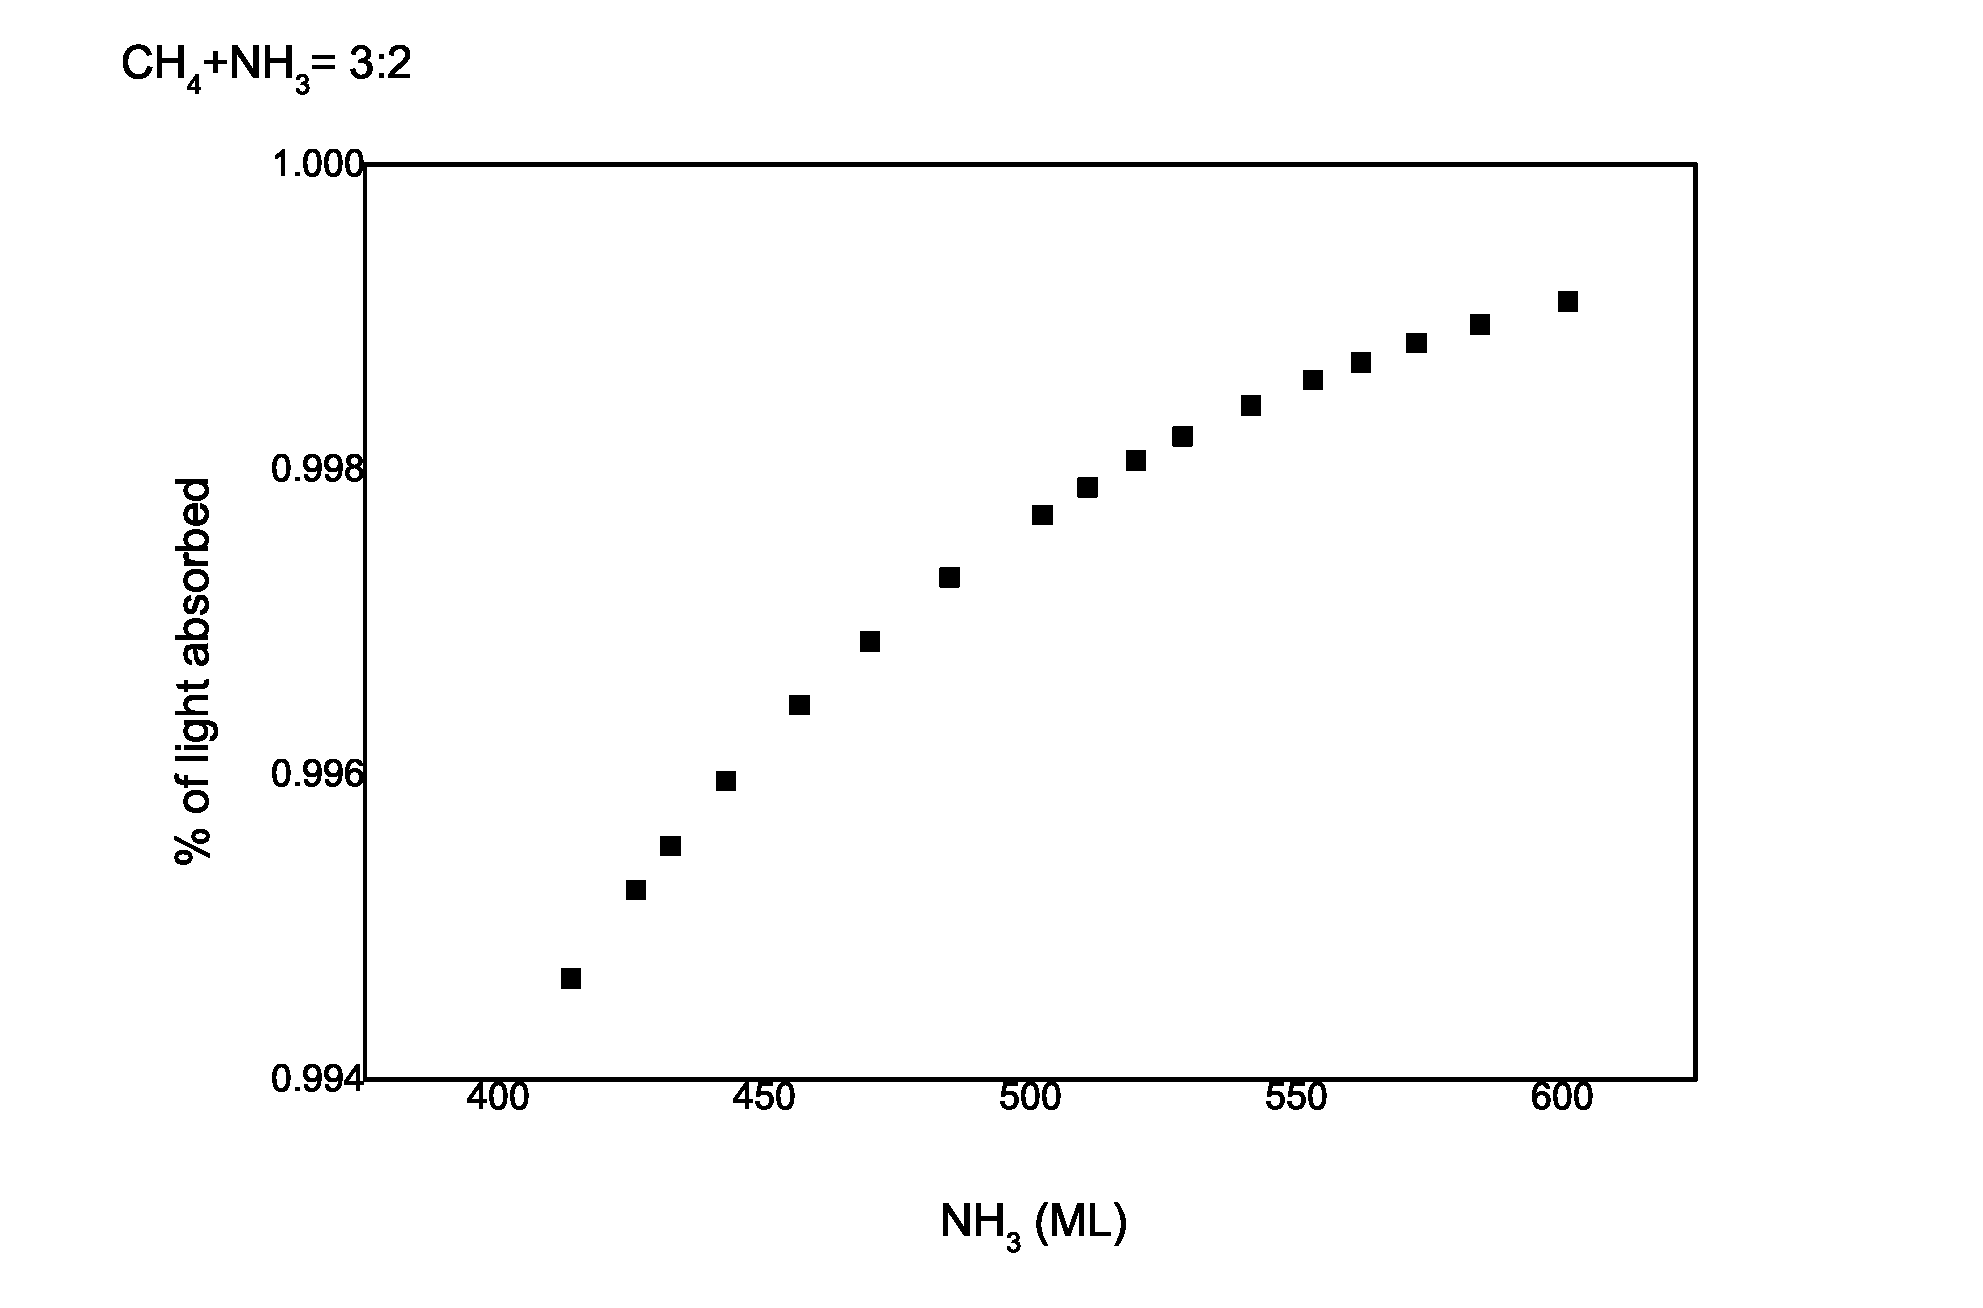
\includegraphics[width=\textwidth]{figures/chapter4/absorption.eps}
\caption{The calculated percentage of VUV irradiation absorbed by different thickness of CH$_4$ to NH$_3$ = 3:2 ice mixtures.}
\label{fig:absorption_percentage}
\end{figure}

\section{Cyanide ion produced by photon sources and electrons} %comparison with Kim use beer's law to get the total irradiated ice 

Considering the ice mixtures in which CH$_4$ is dominated, the efficiencies in CN$^-$ formation by electrons and VUV irradiations is calculated by the final column densities divided by the column densities of the limiting reactant. A fixed amount of CN$^-$ is obtained after irradiations. In our MDHL experiments, we have 14.8 ML of CN$^-$ obtained in (CH$_4$ = 900 ML, NH$_3$= 600 ML) ice mixtures. Kim and Kaiser (2011) irradiated  ice mixtures(CH$_4$ = 610 ML, NH$_3$= 260 ML) and obtained 13 - 16 ML of CN$^-$ adopting the CN$^-$ absorption coefficient (3.7 $\times$ 10$^{-18}$ cm molecule$^{-1}$) \cite{georgieva2006computational}, which is 4.86 times smaller than the absorption strength we adopted. We do not adopt the same absorption coefficient because the number of CN$^-$ produced will exceed CH$_4$ consumption. If we adopted the same absorption coefficient, the production yield of CN$^-$ should be multiplied by 4.86. Therefore, our yield is 72 ML of CN$^-$. Regarding percentage of NH$_3$ (limiting reactant), Kim and Kaiser has 5 - 6 \% yield where we have 12 \% yield if we adopted the same absorption coefficients. 

The above situation is ideal to apply on the slow depositing ices or very thick ices, where photons or electrons can irradiate the surface without renewal. For fast depositing ices, this case is not suitable because only the first few layers are irradiated (figure \ref{fig:absorption_percentage}). The depositing (hitting) rates of CH$_4$ onto the surface of Charon, shown in figure \ref{fig:charon_distribution}, varies from 2 to 6 $\times$ 10$^{11}$ m$^{-2}$ s$^{-1}$ due to the tidal locked rotation of Pluto and charon. In 1 pluto winter (130 earth years), around 110 ML of CH$_4$ will be deposited onto the pole positions, and 3 times more abundant than that at the pole positions facing pluto. This deposition rate is a slow depositing ice because from our experiments: figure \ref{fig:CN_NSRRC}, after 4 $\times$ 10 $^{17}$ VUV photons (about 1 Pluto year), maximum CN$^-$ is formed.  

As a result, under winter time, If we only consider VUV photon source, assuming ratio of CH$_4$ to NH$_3$ is 3:2, about 15 ML of CN$^-$ will be formed during winter time, leading to similar residues as Titan.


\section{Conclusion}
Through investigating methane(CH$_4$) and ammonia(NH$_3$) ice mixtures, we better understand the followings relations: 1. The formation yield of cyanide ion (CN$^-$) is not proportional to the initial deposited methane when methane is dominating. However, the formation rate is proportional to its initial CH$_4$ to NH$_3$ ratios. The competition between CH$_3$ radicals (forming both CH$_3$NH$_2$ and C$_2$H$_6$) and NH$_2$ radicals (forming CH$_3$NH$_2$) results the former result. 2. When VUV is replaced by 40.8 eV 30.4nm He II EUV irradiations, the destruction cross-section of CH$_4$ and NH$_3$ are reduced by  6.06$\pm$0.07 and 3.19$\pm$0.12 times respectively. The lower formation rate of CN$^-$ in EUV irradiation by 3.06 to 4.13 times is mainly due to the reduced NH$_3$ destruction cross-sections. 3. The photo fragmentation of CH$_4$ by more energetic photons are more likely to form C$_3$H$_8$ than C$_2$H$_6$, may infer there are new reaction mechanism pathways (with higher energy barrier) involved to produce C$_3$H$_8$. 4. The functional groups of residues obtained in CH$_4$ to NH$_3$ = 3:2 ice mixtures are similar to the laboratory made Titan tholins.

